\subsubsection{NVIDIA V100 Streaming Multiprocessor (SM)}

The NVIDIA V100 is a powerful GPU designed for data centers, primarily used for Artificial Intelligence (AI), High Performance Computing (HPC), and data science. Meanwhile, the \definition{NVIDIA V100 Streaming Multiprocessor (SM)} is a key component of the V100 GPU architecture.

\highspace
\begin{flushleft}
    \textcolor{Green3}{\faIcon{question-circle} \textbf{How is architecture composed?}}
\end{flushleft}
\begin{itemize}
    \item \textbf{Warp Selector and Fetch/Decode}:
    
    The \emph{Warp Selector} and \emph{Fetch/Decode} units are responsible for \textbf{managing the execution of warps} (groups of threads) and \textbf{decoding instructions}.


    \item \textbf{Functional Units}:
    \begin{itemize}
        \item \definitionWithSpecificIndex{SIMD fp32 functional unit}{NVIDIA V100 SM SIMD fp32 functional unit}{} (Yellow).
        
        It \textbf{handles single-precision floating-point operations}. Control is shared across 16 units, allowing for 16 multiply-add (\texttt{MUL-ADD}) operations per clock cycle. This translates to one 32-wide SIMD operation every two clocks.


        \item \definitionWithSpecificIndex{SIMD int functional unit}{NVIDIA V100 SM SIMD int functional unit}{} (Orange). 
        
        It \textbf{manages integer operations}, also shared across 16 units, with the same performance characteristics as the fp32 unit (16 $\times$ \texttt{MUL-ADD} per clock).
        

        \item \definitionWithSpecificIndex{SIMD fp64 functional unit}{NVIDIA V100 SM SIMD fp64 functional unit}{} (Brown). 
        
        It is \textbf{responsible for double-precision floating-point operations}. Control is shared across 8 units, allowing for 8 \texttt{MUL-ADD} operations per clock cycle, equating to one 32-wide SIMD operation every four clocks.
        

        \item \definitionWithSpecificIndex{Tensor core unit}{NVIDIA V100 SM Tensor core unit}{} (Red). 
        
        It is \textbf{specialized for tensor operations}, which are crucial for deep learning and AI workloads.
        

        \item \definitionWithSpecificIndex{Load/store unit}{NVIDIA V100 SM Load/store unit}{} (Green). 
        
        It \textbf{handles memory operations}, such as loading data from and storing data to memory.
    \end{itemize}


    \item \textbf{Warp Scheduler}:

    The diagram below shows the scheduling of warps (Warp 0, Warp 4, Warp 60, etc.) across the functional units, indicating how different warps are processed in parallel.
\end{itemize}

\newpage

\begin{figure}[!htp]
    \centering
    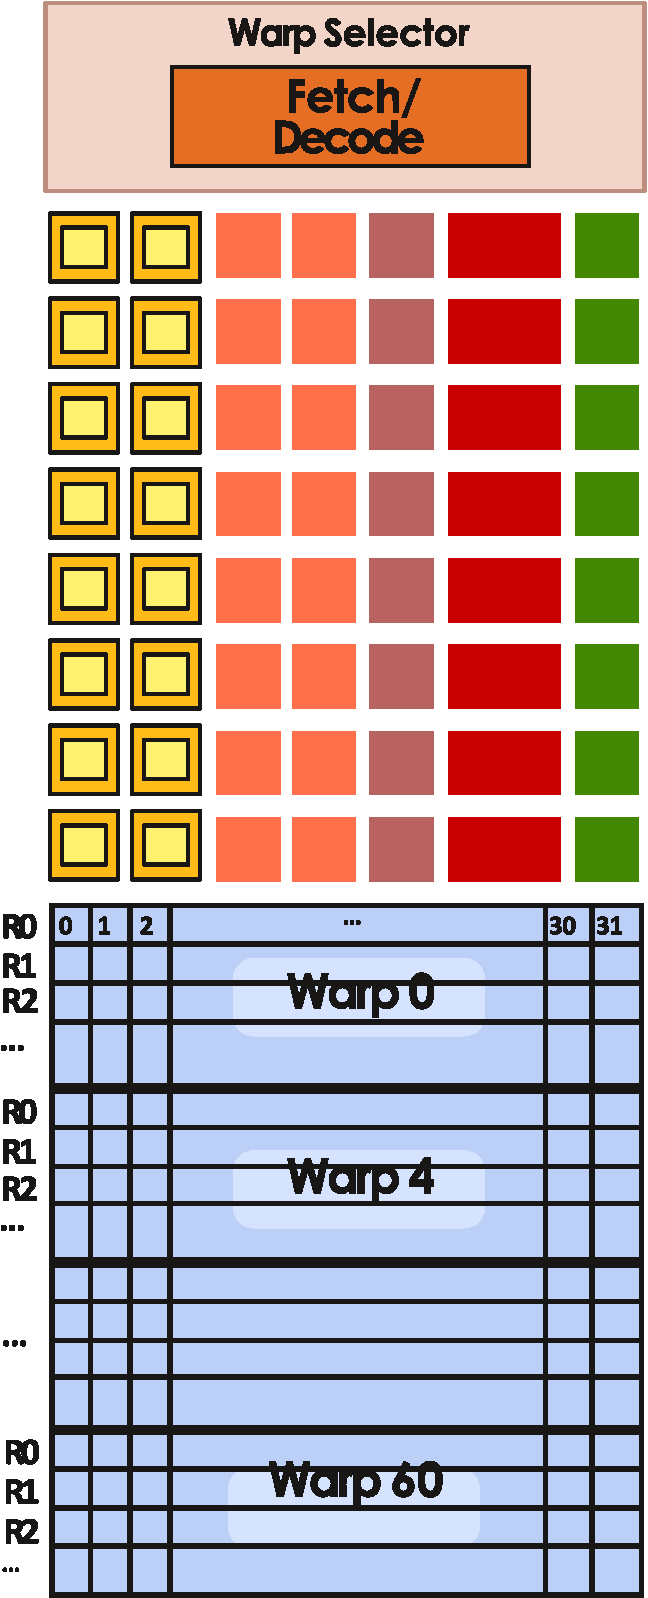
\includegraphics[width=.4\textwidth]{img/nvidia-v100-sm-1.pdf}
    \caption{A \dquotes{sub-core} of the NVIDIA V100 Streaming Multiprocessor (SM) architecture.}
\end{figure}

\begin{flushleft}
    \textcolor{Green3}{\faIcon{question-circle} \textbf{What is a Warp?}}
\end{flushleft}
A \definition{Warp} is a \textbf{group of 32 threads that execute the same instruction at the same time}. \textbf{Threads within a block are divided into warps}. For example, a block of 256 threads would have 8 warps (256 threads / 32 threads per warp). \textbf{Each SM} in the V100 \textbf{can schedule and interleave the execution of up to 16 warps}. This means that multiple warps can be executed simultaneously, improving the overall throughput of the GPU. Finally, each warp has some registers to store the data needed by the threads.

\newpage

\begin{flushleft}
    \textcolor{Green3}{\faIcon{question-circle} \textbf{How is a Warp executed?}}
\end{flushleft}
\textbf{Threads within a warp execute the same instruction simultaneously}, taking advantage of \textbf{SIMD execution} to improve performance. 

\highspace
\textbf{When threads within a warp do not share the same instruction, it results in divergent execution, which can degrade performance due to the need to serialize instructions}. However, the \textbf{check} of the same instruction by the 32 threads is done \textbf{dynamically by the GPU hardware}. Finally, although not part of CUDA, understanding warps is critical to optimizing CUDA programs on modern NVIDIA GPUs.

\highspace
\begin{figure}[!htp]
    \centering
    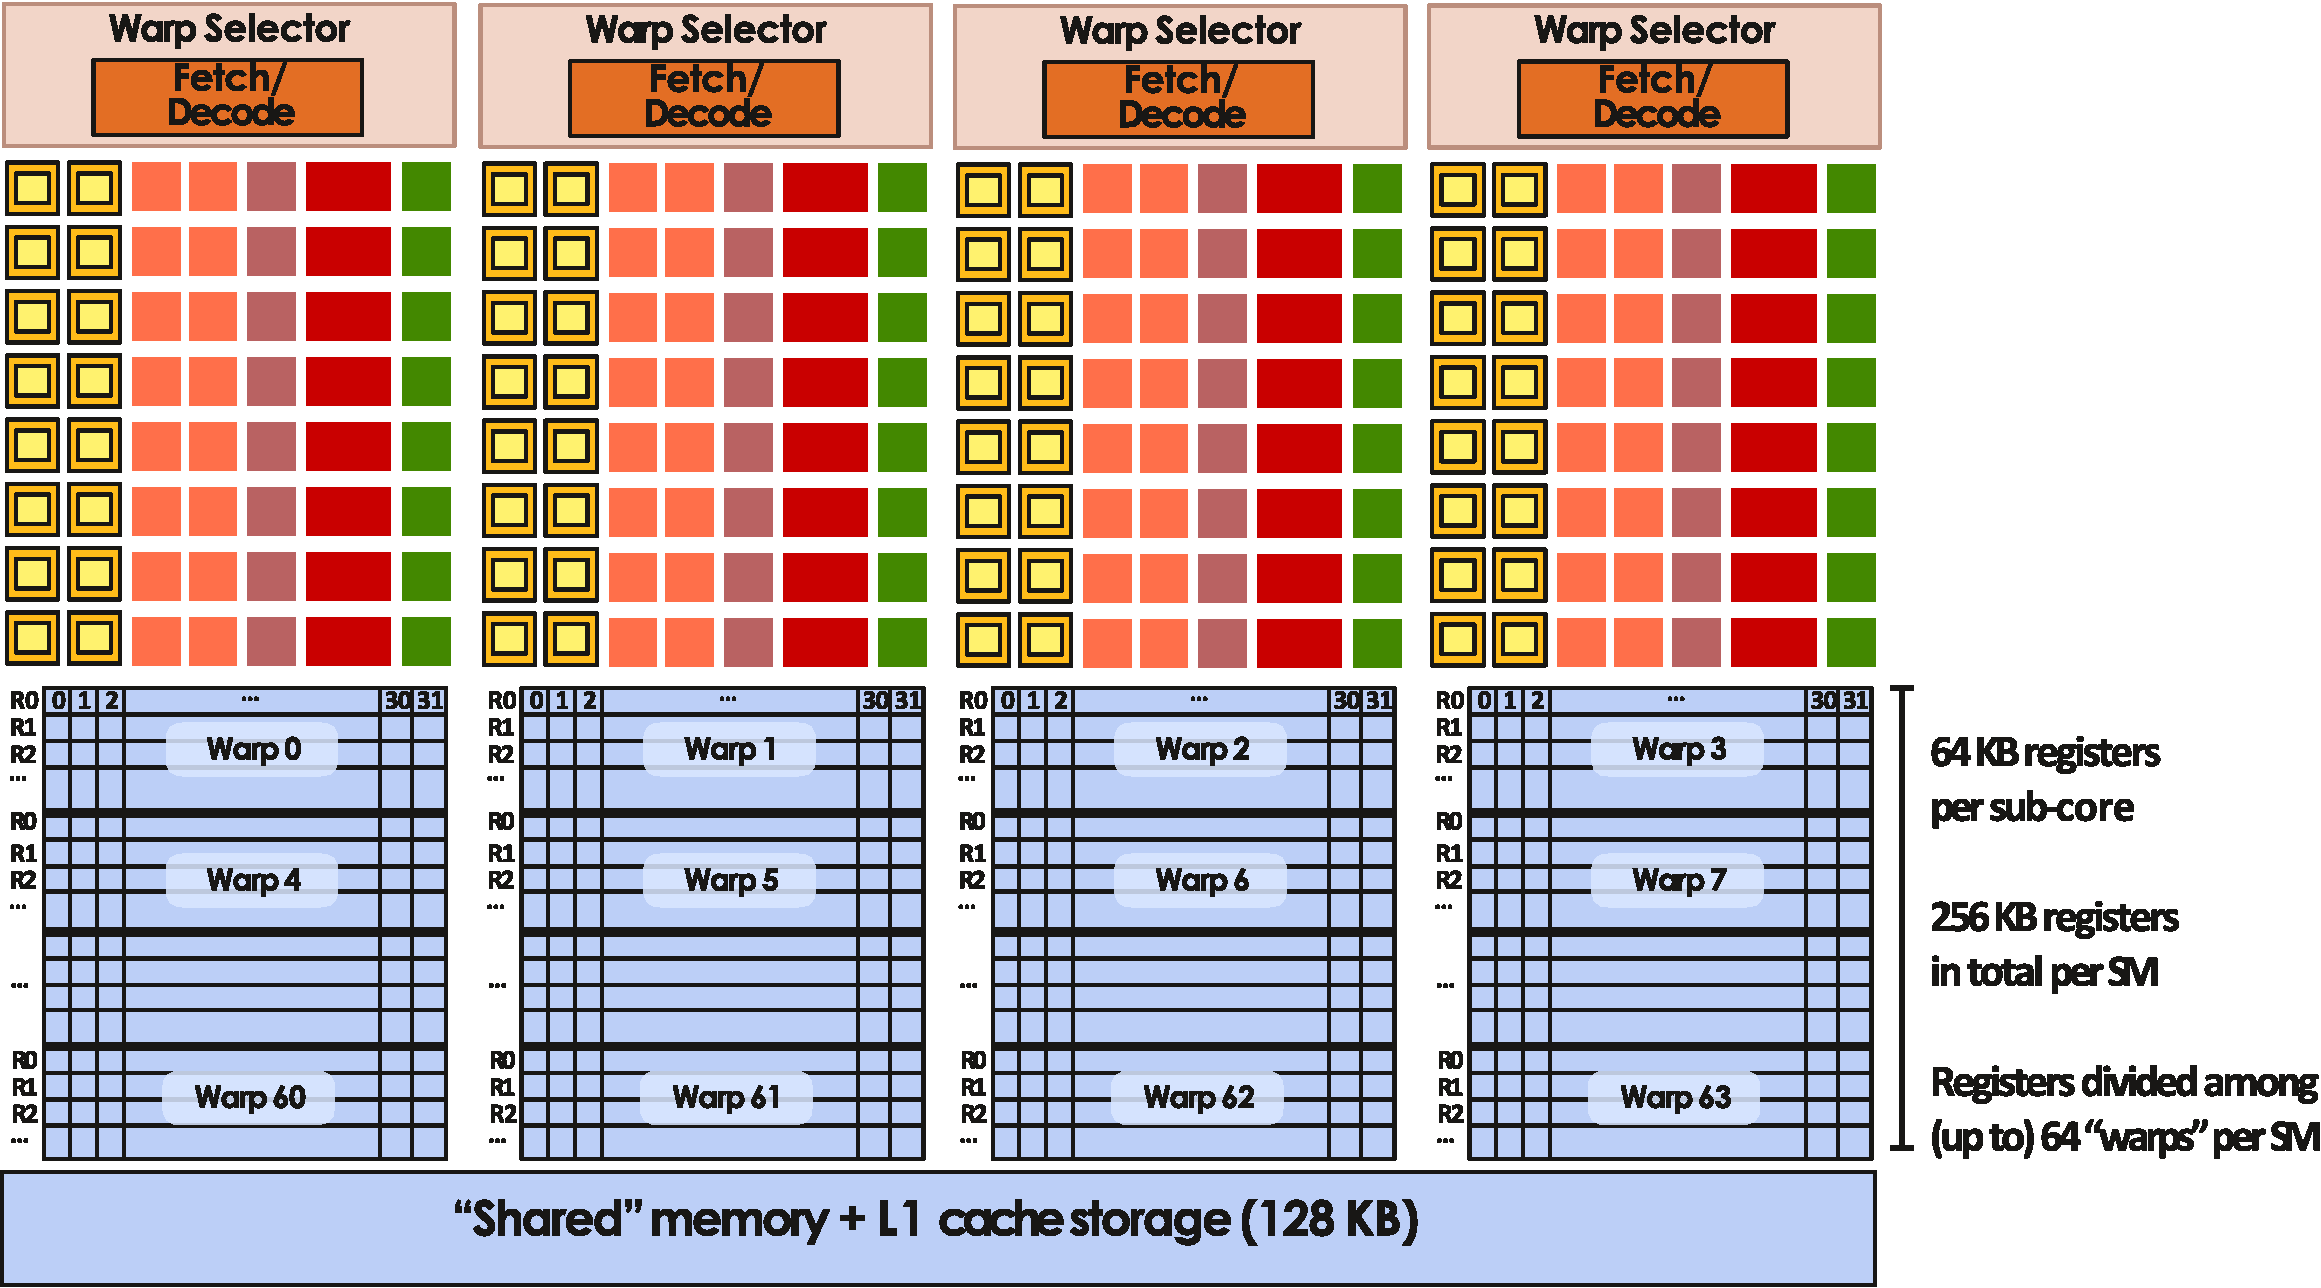
\includegraphics[width=\textwidth]{img/nvidia-v100-sm-2.pdf}
    \caption{A NVIDIA V100 Streaming Multiprocessor (SM) architecture.}
\end{figure}
